\documentclass{article}

\usepackage{../mathclub}

\title{Length Structures} 
\author{}
\date{April 11, 2022}

\begin{document}

\section{Introduction} 
Welcome to Math Club week 3! Today, we will take a look at length structures and rectifiable curves, which are important in metric geometry.  

References: chapter $1$ of ``Metric Structures for Riemannian and Non-riemannian Spaces'' by Gromov and chapter $2$ of ``A Course in Metric Geometry'' by Burago, Burago, and Ivanov.

\section{Fun Exercises} 

\begin{exercise}
Consider the union of segments 
\[\bigcup_{i = 1}^{\infty} [(0, 0), (\cos 1/i, \sin 1/i)] \cup [(0, 0), (1, 0)]
\]
in $\mathbb{R}^{2}$ with the topology inherited from $\mathbb{R}^{2}$. Prove that this topological space is not homeomorphic to a length space. 
\end{exercise}

\begin{center}
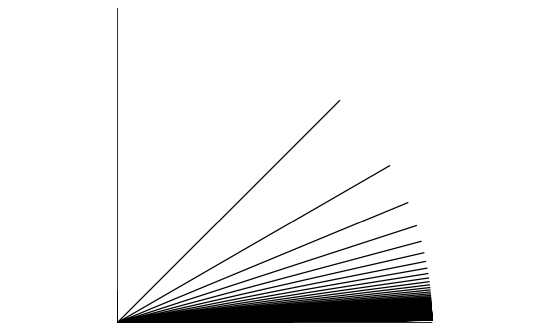
\includegraphics[scale=0.5]{Pics/1.png}
\end{center}

\begin{exercise}
Prove that the intrinsic metric induced by the restriction of Euclidean distance to the circle $x^{2} + y^{2} = 1$ is the angular metric. 
\end{exercise}

\begin{exercise}
Find the induced intrinsic metric for the metric 
\[
d((x_{1}, y_{1}), (x_{2}, y_{2})) = |x_{1} - x_{2}| + \sqrt{|y_{1} - y_{2}|} \]
on $\mathbb{R}^{2}$. What is the topology of the resulting length space?
\end{exercise}

\end{document}